\subsection{Setup}\label{setup}
This chapter explains features which were not implemented as the project was started. These features are mainly chosen in order to grow the community, as offering features as making starting coding with Dafny easier and supporting a wide range of IDEs accomplishes this goal.
\subsubsection{Language Server} \label{setupLanguageServer}
\paragraph{What is a Language Server}
A language server allows to integrate features like auto completion, go to definition, find all references in an easy way into an IDEs. Such a server mostly coexists with a client, which is a normally a native IDE plugin, which does the customization of the GUI, registers shortcuts or adds menu items. The language server provides a list of supported actions, which are normally shown in the IDE. This makes it very handy to extend it as well. 
The protocol between these two components is standardized by Microsoft, with the idea behind it to achieve IDE independence. 
 \newline
\begin{figure}[H]
	\centering
	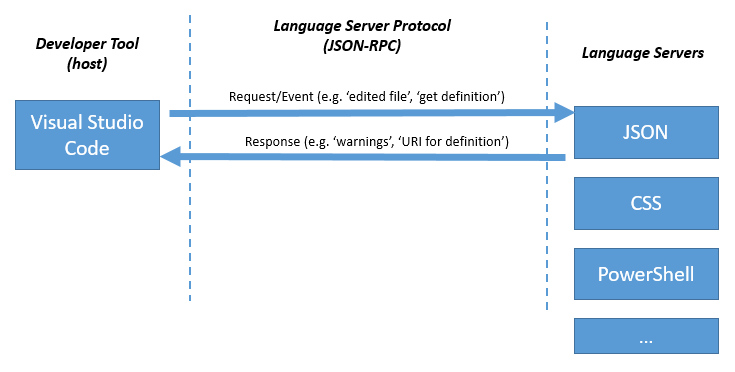
\includegraphics[width=1.0\textwidth]{img/languageServer}
	\caption{Language Server}
	\label{fig:languageServer}
\end{figure}
\paragraph{Why were they chosen to implement}
Since Dafny is already supported on different operation systems, it was decided to make the plugin as platform and IDE independent as possible. Because Visual Studio Code supports the Language Server Protocol and is the reference implementation, the plugin developed by Jonathan Rionatan was refactored to work as a language server. The strict splitting of the plugin into a client and a server had also the benefit, that the architecture had to be changed, which resulted in a much better and clearer structure. \newline
In the future another IDE could just integrate the existing language server, make smaller tweaks to the client and it would work. No rewriting of the whole logic is needed, as one just can use the server, thanks to the standardized protocol. 
\paragraph{What benefits do they entail}
Developing the plugin as a language server has the big benefit, that it could be easily integrated into existing IDEs, which support the Language Server Protocol, without reprogramming everything. Supporting auto completion, go to definition, find all references, would just work, without writing a single line of code. The only step is to start the Language Server and connect to it. Only the client needs to be adjusted, depending on the requirements of how the GUI should look like and probably the programming language to developing the client will change. 
See \ref{ides} for a overview of IDEs which were looked at. 
\subsubsection{Automatic Installation} \label{setupAutomaticInstallation}
\paragraph{What is Automatic Installation}
Automatic Installation is the process to setup the whole Dafny environment in the background. Downloading the latest release from GitHub, extract it and setting all necessary configuration properties correctly is its main task. This process is platform dependent, because there is a zip file for each operating system. 
\paragraph{Why was this chosen to implement}
The setup to start coding with Dafny was quite complicated. The whole installation was not straightforward. First one had to download the Dafny.zip from GitHub, which is hidden under releases. Second it had to be extracted into a directory. Afterwards installing the Dafny plugin for Visual Studio Code and setting the path to the DafnyServer.exe had to be done. Finally after a restart of Visual Studio Code it maybe worked. \newline
Because this is quite complicated, especially if one wants to grow the community, this process must be much easier. For this reason it was decided to implement this important feature. The goal was that a new user can start coding in under 1 minute. 
\paragraph{What benefits do this entail}
More people can start writing Dafny programs, not worrying about having to set up Dafny, struggling with configurations or not finding the release on GitHub. Also professors can integrate Dafny into their lectures, as long as students can install Dafny without problems. 
\subsubsection{Automatic Upgrade} \label{setupAutomaticUpgrade}
\paragraph{What is Automatic Upgrade}
Automatic upgrade makes sure that always the latest version of Dafny is used. If a new release is published on GitHub this feature will check that, and notify the user that there is newer release available. If the user wants to upgrade the Dafny environment, the feature \ref{setupAutomaticInstallation} will take over. 
\paragraph{Why was this chosen to implement}
Most people will never look at GitHub to check if there is a newer version of Dafny available. Especially if there is no need to, because everything can be installed automatically. Out of this reason, there needs to be a version check, which informs the user if there is a newer version. 
\paragraph{What benefits do this entail}
Newer versions bring important bug fixes and new features, which would not be used if there is no version check. Users can install newer version the same easy way, as installing the environment the first time.  
